\chapter{Spesiasi dan Makroevolusi}\label{ch:b2:speciation}

Di sebuah pulau kecil di Galapagos, pada tahun 1982, beberapa ekor
burung pipit tanah berparuh besar tiba dari sebuah pulau tetangga lalu
menetap. Selama dua puluh tahun mereka bersaing dengan burung pipit
tanah sedang yang sudah bermukim di sana untuk memperebutkan \omterm{def:b2:angiosperm-reproduction:seed}{biji} besar
yang disukai keduanya; lalu sebuah kekeringan melanda, \omterm{def:b2:angiosperm-reproduction:seed}{biji} besarnya
menipis, dan penduduk yang berparuh lebih besar --- yaitu yang paling
langsung bersaing dengan pendatangnya --- kelaparan. Dalam satu
generasi paruh penduduknya telah menyusut, secara terukur, menjauhi
paruh penyerbunya. Dua spesies yang telah berjumpa didorong saling
menjauh. Bab ini membahas pembuatan spesies: apa itu sebuah spesies dan
apa yang menjaganya tetap khas, bagaimana satu populasi menjadi dua,
persaingan yang mendorong populasi saling menjauh ketika mereka
berjumpa, dan pandangan panjang catatan fosilnya, yang di dalamnya
proses yang sama yang diulang seratus juta kali memberikan pohon
kehidupan.

\section{Apa itu sebuah spesies}

\begin{definition}[Spesies]\label{def:b2:speciation:species}
\index{konsep spesies}\index{konsep spesies biologis}\index{pengisolasian reproduktif}
Menurut \emph{konsep spesies biologis}, sebuah spesies adalah
sekelompok populasi yang anggotanya dapat saling mengawini dan
menghasilkan keturunan yang subur, serta \emph{terisolasi secara
reproduktif} dari kelompok lain semacam itu: yang menyatukan sebuah
spesies adalah \omterm{prop:b2:population-genetics:migration}{aliran gen}, dan yang memisahkan spesies adalah
ketiadaannya. Konsepnya berhasil bagi jasad seksual pada satu zaman dan
satu tempat, yang merupakan sebagian besar dari yang dijumpai seorang
ahli biologi; konsepnya gagal bagi garis keturunan aseksual (yang
dinamai menurut kemiripannya), bagi fosil (yang tidak dapat
disilangkan), dan bagi banyak kasus yang batasnya bocor --- pohon ek
dan pohon dedalu yang berhibrida lintas spesies, itik yang spesiesnya
saling mengawini dalam kurungan, spesies cincin yang di dalamnya
populasi tetangga saling mengawini sepanjang jalan mengelilingi sebuah
penghalang sampai kedua ujungnya berjumpa lalu tidak. Konsep lain
mengisi celahnya: spesies \emph{morfologis} (sebuah gugus bentuk yang
serupa), spesies \emph{filogenetik} (garis keturunan terkecil yang
dapat didiagnosis), spesies \emph{ekologis} (sebuah garis keturunan
yang menempati relungnya sendiri). Tidak ada yang salah;
masing-masingnya mengukur sesuatu yang nyata, dan spesiasi adalah
proses yang dengannya semuanya menjadi sepakat.
\end{definition}

\begin{proposition}[Mekanisme pengisolasi]\label{prop:b2:speciation:isolation}
\index{mekanisme pengisolasi}\index{pengisolasian prazigotik}%
\index{pengisolasian pascazigotik}\index{kaidah Haldane}
\omterm{prop:b2:population-genetics:migration}{Aliran gen} antara dua populasi dihentikan penghalang yang bekerja
sebelum atau sesudah pembuahannya. \emph{Prazigotik}: populasinya hidup
di habitat yang berbeda atau berbiak pada musim yang berbeda
(pengisolasian waktu: dua ekor katak yang memanggil pada bulan yang
berbeda); populasinya tidak mengenali pacaran satu sama lain (perilaku:
nyanyian jangkrik, sandi cahaya kunang-kunang, tarian itik); alat
kelamin atau \omterm{def:b2:angiosperm-reproduction:flower}{bunganya} tidak cocok (mekanis); gametnya tidak melebur
(gametik: protein pengikat sperma bulu babi, \omterm{def:b2:meiosis-heredity:vocabulary}{alel} $S$ pada
\cref{ch:b2:angiosperm-reproduction}). \emph{Pascazigotik}: hibridanya
mati sebagai embrio, atau hidup tetapi mandul (bagal; hibrida dua
spesies \emph{Drosophila}), atau subur tetapi keturunannya sendiri
tidak (keruntuhan hibrida). \emph{\omterm{prop:b2:speciation:isolation}{Kaidah Haldane}}: ketika hanya satu
jenis kelamin hibridanya yang mandul atau tidak dapat hidup, jenis
kelamin itu adalah yang memiliki dua \omterm{prop:b2:meiosis-heredity:sexlinked}{kromosom kelamin} yang berbeda ---
jantan pada mamalia dan lalat, betina pada burung dan kupu-kupu ---
karena ketaksesuaian \omterm{def:b2:meiosis-heredity:vocabulary}{resesif} pada kromosom X tersingkap padanya.
Penghalang prazigotiknya lebih murah, karena tidak ada gamet yang
terbuang, dan seleksi membangunnya di tempat penghalang pascazigotiknya
sudah ada.
\end{proposition}

\begin{theorem}[Mengapa hibridanya gagal: model dua lokus]\label{thm:b2:speciation:dm}
\index{ketaksesuaian Dobzhansky--Muller}
Dua populasi bermula dengan \omterm{def:b2:meiosis-heredity:vocabulary}{genotipe} $aabb$. Pada yang satu, $a$
digantikan $A$; pada yang lain, $b$ digantikan $B$; tiap penggantiannya
netral atau menguntungkan pada latarnya sendiri, sehingga tak satu pun
populasinya pernah melewati sebuah keadaan yang kurang bugar. Tetapi
$A$ dan $B$ tidak pernah diuji bersama-sama, dan jika gabungannya tidak
sesuai --- jika protein yang dibuat $A$ tidak dapat bekerja dengan
protein yang dibuat $B$ --- hibrida $AaBb$-nya tidak bugar. Karena itu
\omterm{def:b2:speciation:species}{pengisolasian reproduktif} muncul sebagai hasil sampingan pemencarannya,
tanpa lembah yang diseberangi dan tanpa seleksi bagi pengisolasiannya
sendiri; dan karena tiap penggantian baru pada satu garis keturunan
dapat tidak sesuai dengan tiap penggantian yang sudah terpancang pada
garis keturunan yang lain, jumlah ketaksesuaian yang mungkin bertambah
sebagai \emph{kuadrat} jumlah penggantiannya --- pengisolasiannya
\emph{membola salju} bersama waktu.
\end{theorem}
\begin{proof}
Dengan $n$ penggantian pada tiap garis keturunannya, masing-masing dari
$n$ \omterm{def:b2:meiosis-heredity:vocabulary}{alel} baru satu garis keturunan boleh jadi tidak sesuai dengan
masing-masing dari $n$ \omterm{def:b2:meiosis-heredity:vocabulary}{alel} garis keturunan yang lain: $n^{2}$ pasang,
yang masing-masingnya tidak sesuai dengan suatu peluang $\varepsilon$,
sehingga jumlah harapan ketaksesuaiannya adalah $\varepsilon n^{2}$,
dan $n$ bertambah bersama waktu sejak pembelahannya. Hibridanya adalah
satu-satunya \omterm{def:b2:meiosis-heredity:vocabulary}{genotipe} yang kedua perangkatnya berjumpa di dalamnya.
\end{proof}
\begin{proof}[Bukti eksperimental]
Coyne dan Orr (1989, 1997) menghimpun ratusan pasang spesies
\emph{Drosophila} yang jarak genetiknya diketahui (yaitu sebuah ukuran
waktu sejak pemencarannya) lalu mengukur \omterm{prop:b2:speciation:isolation}{pengisolasian prazigotik} dan
pascazigotiknya: keduanya naik bersama jaraknya, pengisolasiannya pada
dasarnya lengkap pada sebuah jarak yang bersesuaian dengan beberapa
juta tahun, dan pasangan yang hidup di daerah yang sama menunjukkan
\omterm{prop:b2:speciation:isolation}{pengisolasian prazigotik} yang lebih kuat pada sebuah jarak tertentu
daripada pasangan yang tidak --- yaitu tanda tangan penguatannya. Gen
ketaksesuaiannya telah dikenali satu demi satu sejak itu, dan jumlah
yang ditemukan antara dua spesies memang bertambah lebih cepat daripada
lurus bersama pemencarannya.
\end{proof}

\begin{omfigure}
\begin{tikzpicture}[every node/.style={font=\scriptsize}, >=stealth]
  \node[draw, rounded corners, fill=omExo!25] (anc) at (0,0) {moyang $aabb$};
  \node[draw, rounded corners, fill=omDef!15] (p1) at (-2.6,-1.8) {populasi 1: $AAbb$};
  \node[draw, rounded corners, fill=omThm!15] (p2) at (2.6,-1.8) {populasi 2: $aaBB$};
  \node[draw, rounded corners, fill=gray!25, align=center] (hyb) at (0,-3.6) {hibrida $AaBb$:\\$A$ dan $B$ berjumpa untuk pertama kalinya\\--- tidak sesuai, tidak bugar};
  \draw[->, thick] (anc) -- (p1) node[midway, left, align=right] {$a \to A$ terpancang,\\bugar pada latarnya};
  \draw[->, thick] (anc) -- (p2) node[midway, right, align=left] {$b \to B$ terpancang,\\bugar pada latarnya};
  \draw[->, thick] (p1) -- (hyb); \draw[->, thick] (p2) -- (hyb);
  \node[anchor=west, align=left, text width=4.6cm] at (4.6,-0.4) {tak satu pun populasinya menyeberangi sebuah lembah; pengisolasiannya adalah hasil sampingan, dan jumlah pasangan semacam itu bertambah sebagai $n^{2}$};
\end{tikzpicture}

{\small Model dua lokus kegagalan hibridanya. Tiap populasinya
memancangkan sebuah perubahan yang bekerja pada latarnya sendiri;
hibridanya adalah \omterm{def:b2:meiosis-heredity:vocabulary}{genotipe} pertama yang menggabungkan keduanya.}
\end{omfigure}

\section{Bagaimana satu spesies menjadi dua}

\begin{proposition}[Modus spesiasi]\label{prop:b2:speciation:modes}
\index{spesiasi alopatrik}\index{spesiasi simpatrik}%
\index{spesiasi parapatrik}\index{efek pendiri}
Spesiasi \emph{alopatrik} bermula dengan sebuah penghalang geografis:
sebuah sebaran yang terbelah gunung yang naik, sebuah laut yang
mengering, atau sebuah sungai baru (\emph{vikarians}), atau beberapa
penjajah yang terbawa ke sebuah pulau (\emph{peripatrik}, beserta \omterm{prop:b2:speciation:modes}{efek
pendiri} dan hanyutan pada \cref{ch:b2:population-genetics}). Terputus
dari \omterm{prop:b2:population-genetics:migration}{aliran gennya}, kedua populasinya memencar lewat seleksi di
lingkungan yang berbeda, lewat hanyutan, dan lewat \omterm{def:b2:genome-diversification:mutation}{mutasinya}
masing-masing, sampai ketaksesuaiannya menimbun; jika keduanya berjumpa
lagi keduanya tidak lagi melebur. Itulah modus yang paling lazim, dan
pola spesies bersaudara pada sisi yang berlawanan dari tiap tanah
genting, barisan gunung, dan selat adalah catatannya. Spesiasi
\emph{simpatrik} terjadi tanpa sebuah penghalang: dalam satu langkah
lewat \omterm{def:b2:genome-diversification:polyploidy}{poliploidi} (\cref{ch:b2:genome-diversification}) --- sepertiga
spesies tumbuhan muncul dengan cara ini; atau lewat seleksi pemecah
dengan perkawinan berpilih, ketika sebuah populasi memanfaatkan dua
sumber daya dan individunya mengawin pada sumber daya yang ia pakai
(lalat belatung apel yang berpindah dari hawthorn ke apel pada tahun
1860-an dan kini mengawin pada inangnya; ikan siklid sebuah danau
kawah). Spesiasi \emph{parapatrik} terjadi sepanjang sebuah landaian
lingkungan, yang padanya sebuah populasi beradaptasi dengan kedua
ujungnya dan sebuah \omterm{prop:b2:speciation:reinforcement}{zona hibrida} terbentuk di tengahnya. Pada tiap
modusnya resepnya sama: kurangi \omterm{prop:b2:population-genetics:migration}{aliran gennya}, biarkan pemencarannya
menimbun, dan biarkan hasil sampingan pemencarannya menjadi penghalang.
\end{proposition}

\begin{omfigure}
\resizebox{\linewidth}{!}{%
\begin{tikzpicture}[every node/.style={font=\scriptsize}, >=stealth]
  \foreach \x/\lab in {0/{alopatrik:\\sebuah penghalang membelah sebarannya}, 5.2/{peripatrik:\\beberapa pendiri di sebuah pulau}, 10.4/{simpatrik:\\dua inang, mengawin pada inangnya}} \node[align=center, anchor=south] at (\x+1.8,3.0) {\lab};
  % allopatric
  \draw[thick, fill=omDef!15] (0.9,1.4) ellipse (0.8 and 0.9);
  \draw[thick, fill=omThm!15] (2.7,1.4) ellipse (0.8 and 0.9);
  \draw[very thick, omExo!70!black] (1.8,0.2) -- (1.8,2.6);
  \node[below] at (1.8,0.1) {gunung, laut, sungai};
  % peripatric
  \begin{scope}[xshift=5.2cm]
    \draw[thick, fill=omDef!15] (1.0,1.4) ellipse (1.0 and 0.9);
    \draw[thick, fill=omThm!15] (3.2,1.9) circle (0.35);
    \draw[->, thick, dashed] (2.0,1.6) -- (2.85,1.85);
    \node[below] at (3.2,1.5) {pendiri};
    \node[below] at (1.0,0.4) {daratan};
  \end{scope}
  % sympatric
  \begin{scope}[xshift=10.4cm]
    \draw[thick, fill=omExo!15] (1.8,1.4) ellipse (1.7 and 0.9);
    \foreach \p in {(1.0,1.6),(1.3,1.2),(0.8,1.2),(1.2,1.8)} \fill[omDef] \p circle (0.07);
    \foreach \p in {(2.4,1.6),(2.7,1.2),(2.2,1.2),(2.6,1.8)} \fill[omThm] \p circle (0.07);
    \node[omDef, below] at (1.0,0.5) {inang A}; \node[omThm, below] at (2.6,0.5) {inang B};
    \node[below] at (1.8,0.1) {satu tempat, dua sumber daya};
  \end{scope}
\end{tikzpicture}}

{\small Tiga jalan menuju dua spesies: sebuah penghalang yang melintasi
sebarannya, sebuah populasi pendiri di baliknya, atau dua sumber daya
di dalamnya.}
\end{omfigure}

\begin{proposition}[Penguatan dan zona hibrida]\label{prop:b2:speciation:reinforcement}
\index{penguatan (spesiasi)}\index{zona hibrida}\index{klina}
Ketika dua populasi yang telah memencar berjumpa lagi, tiga hal dapat
terjadi. Jika hibridanya sebugar induknya, keduanya melebur. Jika
hibridanya tidak bugar, seleksi menyukai individu yang menolak
mengawin dengan jenis yang lain --- gamet yang terbuang adalah
ongkosnya --- dan \omterm{prop:b2:speciation:isolation}{pengisolasian prazigotiknya} menguat di tempat
keduanya bertindih (\emph{penguatan}), sampai keduanya menjadi spesies.
Di antara keduanya, sebuah \emph{\omterm{prop:b2:speciation:reinforcement}{zona hibrida}} bertahan: sebuah pita,
yang sering lebarnya beberapa kilometer, yang di dalamnya kedua
bentuknya saling mengawini dan hibridanya dihasilkan tiap generasi,
yang dijaga oleh keseimbangan antara pemencaran ke dalam zonanya dan
seleksi terhadap hibridanya di dalamnya. Melintasi zona semacam itu
frekuensi tiap bentuknya mengikuti sebuah \emph{klina}, yaitu sebuah
kurva berbentuk S yang lebarnya $w$ ditetapkan jarak pemencarannya
$\sigma$ tiap generasi dan seleksinya $s$ terhadap hibridanya, $w \approx
\sigma\sqrt{8/s}$: sebuah zona dapat tetap sempit selama ribuan
tahun tanpa kedua bentuknya pernah melebur atau berpisah sepenuhnya.
Kodok, gagak, mencit, dan belalang Eropa memperlihatkan berlusin-lusin
zona semacam itu, yang sebagian besarnya berjalan sepanjang garis
tempat populasi yang telah berlindung di tempat perlindungan yang
terpisah selama zaman es terakhir berjumpa lagi ketika esnya surut.
\end{proposition}
\begin{proof}[Bukti eksperimental]
Di tempat burung sikatan belang dan sikatan berkalung bertindih di
Eropa tengah, jantan tiap spesiesnya memiliki bulu yang lebih berbeda
dari bulu spesies lainnya daripada di tempat keduanya hidup terpisah,
dan betinanya membeda-bedakan dengan lebih tajam --- yaitu penguatan
yang terukur di lapangan. Kodok berperut api dan kodok berperut kuning
berjumpa sepanjang sebuah zona melintasi Polandia yang lebarnya
beberapa kilometer, yang mantap selama ia dipelajari, dengan lebar
klina yang diramalkan dari pemencarannya dan \omterm{def:b2:population-genetics:fitness}{kebugaran} hibridanya yang
berkurang.
\end{proof}

\begin{omfigure}
\begin{tikzpicture}
\begin{axis}[
  width=0.72\linewidth, height=5.2cm,
  axis x line=bottom, axis y line=left,
  xmin=-30, xmax=30, ymin=0, ymax=1.05,
  xlabel={jarak melintasi zonanya (km)}, ylabel={frekuensi bentuk A},
  xlabel style={font=\small, at={(axis description cs:0.5,-0.13)}, anchor=north},
  ylabel style={font=\small},
  tick label style={font=\small}, xtick={-20,-10,0,10,20}, ytick={0,0.5,1},
  clip=false,
]
\addplot[very thick, omDef, domain=-30:30, samples=100] {1/(1+exp(x/2.2))};
\draw[dashed, gray] (axis cs:-4.4,0) -- (axis cs:-4.4,1); \draw[dashed, gray] (axis cs:4.4,0) -- (axis cs:4.4,1);
\draw[<->] (axis cs:-4.4,0.08) -- (axis cs:4.4,0.08); \node[font=\scriptsize, anchor=south] at (axis cs:0,0.09) {lebar $w$};
\node[font=\scriptsize, anchor=west, align=left] at (axis cs:8,0.75) {$w \approx \sigma\sqrt{8/s}$: pemencaran\\$\sigma = \qty{1}{km}$, $s = 0.1$\\memberikan $w \approx \qty{9}{km}$};
\end{axis}
\end{tikzpicture}

{\small Sebuah klina melintasi sebuah \omterm{prop:b2:speciation:reinforcement}{zona hibrida}: frekuensi salah
satu bentuknya turun dari satu menjadi nol sepanjang sebuah lebar yang
ditetapkan seberapa jauh individunya memencar dan seberapa tidak bugar
hibridanya.}
\end{omfigure}

\section{Persaingan, hidup berdampingan, dan pergeseran sifat}

\begin{theorem}[Persaingan Lotka--Volterra]\label{thm:b2:speciation:lv}
\index{persaingan Lotka--Volterra}\index{penyingkiran bersaing}\index{hidup berdampingan}
Dua spesies yang tumbuh secara logistik (jilid Tahun 1) yang bersaing
memperebutkan sebuah sumber daya mematuhi
\[
\frac{\mathrm{d}N_1}{\mathrm{d}t} = r_1 N_1\Bigl(1 - \frac{N_1 + \alpha N_2}{K_1}\Bigr), \qquad
\frac{\mathrm{d}N_2}{\mathrm{d}t} = r_2 N_2\Bigl(1 - \frac{N_2 + \beta N_1}{K_2}\Bigr),
\]
dengan $\alpha$ mengukur efek satu individu spesies 2 terhadap spesies
1 dalam satuan individu spesies 1 sendiri, dan $\beta$ kebalikannya.
Spesies 1 berhenti tumbuh pada garis $N_1 + \alpha N_2 =
K_1$ (yaitu
\emph{isoklinnya}), spesies 2 pada $N_2 + \beta N_1 = K_2$, dan hasilnya
bergantung pada bagaimana kedua garisnya berpotongan:
\begin{itemize}
  \item $K_1 > \alpha K_2$ dan $K_2 < \beta K_1$: spesies 1 selalu
        menang;
  \item $K_1 < \alpha K_2$ dan $K_2 > \beta K_1$: spesies 2 selalu
        menang;
  \item $K_1 > \alpha K_2$ dan $K_2 > \beta K_1$: \emph{\omterm{thm:b2:speciation:lv}{hidup
        berdampingan} yang mantap} pada $N_1^{*} = (K_1 - \alpha K_2)/(1 - \alpha\beta)$,
        $N_2^{*} = (K_2 - \beta K_1)/(1 - \alpha\beta)$;
  \item $K_1 < \alpha K_2$ dan $K_2 < \beta K_1$: salah satunya
        menang, bergantung pada siapa yang bermula lebih banyak.
\end{itemize}
\omterm{thm:b2:speciation:lv}{Hidup berdampingan} menuntut $\alpha\beta < 1$ dengan tiap spesiesnya
lebih tertahan oleh jenisnya sendiri daripada oleh jenis yang lain: dua
spesies yang memakai sumber daya yang persis sama ($\alpha = \beta = 1$) tidak dapat \omterm{thm:b2:speciation:lv}{hidup berdampingan} (yaitu \emph{asas \omterm{thm:b2:speciation:lv}{penyingkiran
bersaing}}), dan makin berbeda apa yang keduanya pakai, makin kecil
$\alpha$ dan $\beta$ serta makin kukuh keduanya \omterm{thm:b2:speciation:lv}{hidup berdampingan}.
\end{theorem}
\begin{proof}
Pada isoklin spesies 1, $\mathrm{d}N_1/\mathrm{d}t = 0$; di bawahnya
(menuju titik asalnya) $N_1$ bertambah, di atasnya $N_1$ turun;
demikian pula bagi spesies 2. Tiap isoklinnya adalah sebuah garis lurus
dengan potongan $K_1$ pada sumbu $N_1$ dan $K_1/\alpha$ pada sumbu
$N_2$ (milik spesies 1), serta $K_2/\beta$ dan $K_2$ (milik spesies 2).
Spesies 1 dapat menyerbu sebuah populasi spesies 2 pada daya dukungnya
$K_2$ jika pertumbuhannya sendiri positif di sana, yakni jika $K_1 > \alpha K_2$; spesies 2 dapat menyerbu spesies 1 pada $K_1$ jika $K_2 > \beta K_1$. Ketika keduanya dapat saling menyerbu, tak satu pun dapat
disingkirkan dan lintasannya menuju perpotongan isoklinnya, yang
ditemukan dengan menyelesaikan kedua persamaan garisnya; ketika hanya
satu yang dapat, yang itulah yang menang; ketika tak satu pun dapat,
perpotongannya adalah sebuah pelana dan pendirinya yang menang.
Kemantapan titik dalamnya menyusul dari hujah penyerbuannya: jika
diusik menuju salah satu sumbunya, spesies yang lebih jarang tumbuh
kembali.
\end{proof}

\begin{omfigure}
\begin{tikzpicture}
\begin{axis}[
  width=0.6\linewidth, height=6cm,
  axis x line=bottom, axis y line=left,
  xmin=0, xmax=1300, ymin=0, ymax=1900,
  xlabel={$N_1$}, ylabel={$N_2$},
  xlabel style={font=\small, at={(axis description cs:0.5,-0.1)}, anchor=north},
  ylabel style={font=\small},
  tick label style={font=\small}, xtick={0,857,1000,1333}, xticklabels={0,$N_1^*$,$K_1$,$K_2/\beta$}, ytick={0,286,800,2000}, yticklabels={0,$N_2^*$,$K_2$,$K_1/\alpha$},
  clip=false,
]
\addplot[very thick, omDef, domain=50:1000, samples=2] {(1000-x)/0.5};
\addplot[very thick, omThm, domain=0:1333, samples=2] {800-0.6*x};
\fill[black] (axis cs:857,286) circle (2.5pt);
\draw[->, thick, gray] (axis cs:150,1750) -- (axis cs:300,1450);
\draw[->, thick, gray] (axis cs:1200,100) -- (axis cs:1000,250);
\draw[->, thick, gray] (axis cs:150,150) -- (axis cs:400,250);
\node[font=\scriptsize, omDef, anchor=west] at (axis cs:700,1000) {isoklin spesies 1};
\node[font=\scriptsize, omThm, anchor=south west] at (axis cs:130,740) {isoklin spesies 2};
\node[font=\scriptsize, anchor=south west] at (axis cs:880,320) {hidup berdampingan yang mantap};
\end{axis}
\end{tikzpicture}

{\small Bidang fase dua pesaing dengan $K_1 = 1000$, $K_2 =
800$, $\alpha = 0.5$, $\beta = 0.6$: tiap spesiesnya dapat menyerbu daya
dukung spesies lainnya, dan lintasannya menuju perpotongan isoklinnya
pada $N_1^{*} = 857$, $N_2^{*} = 286$.}
\end{omfigure}

\begin{proposition}[Pergeseran sifat]\label{prop:b2:speciation:displacement}
\index{pergeseran sifat}\index{relung}\index{radiasi adaptif}
Persaingan bukan hanya sebuah hasil ekologis melainkan juga sebuah gaya
evolusi. Di tempat dua spesies yang serupa berjumpa, individu tiap
spesiesnya yang paling menyerupai spesies lainnya paling menderita
karena persaingannya, dan seleksi mendorong keduanya saling menjauh
dalam sifat yang mengatur pemakaian sumber dayanya --- ukuran paruh,
ukuran tubuh, waktu berbunga: populasi yang bertindih lebih berbeda
daripada populasi yang hidup sendiri. \emph{\omterm{prop:b2:speciation:displacement}{Pergeseran sifat}} ini
memperkecil $\alpha$ dan $\beta$, mengubah sebuah pertarungan menuju
penyingkiran menjadi \omterm{thm:b2:speciation:lv}{hidup berdampingan}, dan, jika diulang sepanjang
sebuah bentang kesempatan, menghasilkan sebuah \emph{\omterm{prop:b2:speciation:displacement}{radiasi adaptif}}:
satu penjajah menjadi selusin spesies yang masing-masing cocok dengan
sebuah sumber daya --- burung pipit Darwin di Galapagos, burung
honeycreeper Hawaii, ikan siklid danau Afrika (lima ratus spesies di
Danau Victoria dalam kurang dari lima belas ribu tahun), kadal anol
Karibia, yang di sana perangkat relung yang sama telah diisi perangkat
bentuk tubuh yang sama secara bebas di empat pulau.
\end{proposition}
\begin{proof}[Bukti eksperimental]
Keluarga Grant mencatat tiap burung pipit di Daphne Major selama empat
puluh tahun. Setelah burung pipit tanah besar memantapkan diri pada
tahun 1982, paruh burung pipit tanah sedangnya tidak berubah sampai
kekeringan tahun 2004, ketika \omterm{def:b2:angiosperm-reproduction:seed}{biji} besarnya menjadi langka dan kedua
spesiesnya bersaing memperebutkannya; burung pipit sedang yang berparuh
terbesar mati secara tak sebanding, dan paruh generasi berikutnya lebih
kecil daripada yang pernah terlihat dalam satu langkah --- yaitu
\omterm{prop:b2:speciation:displacement}{pergeseran sifat} yang diramalkan teori, yang teramati ketika ia
terjadi, beserta diferensial seleksi dan heritabilitasnya yang terukur.
Paruh burung pipit yang sama, yang dibandingkan antara pulau tempat
mereka hidup sendiri dan pulau tempat mereka berjumpa, memperlihatkan
pergeseran yang sama yang tertulis di seluruh kepulauannya.
\end{proof}

\begin{omfigure}
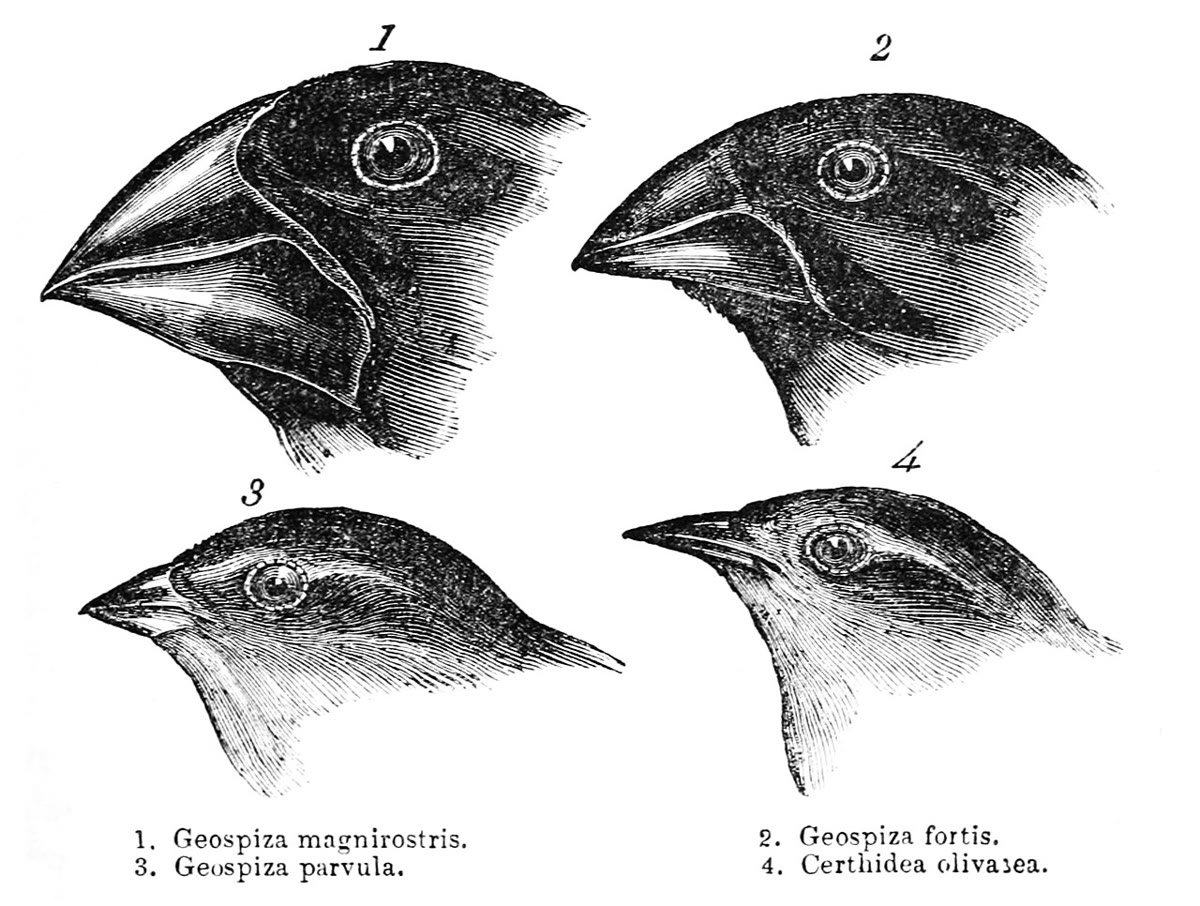
\includegraphics[width=0.44\linewidth]{images/book2/finches-gould.jpg}\hspace{0.04\linewidth}
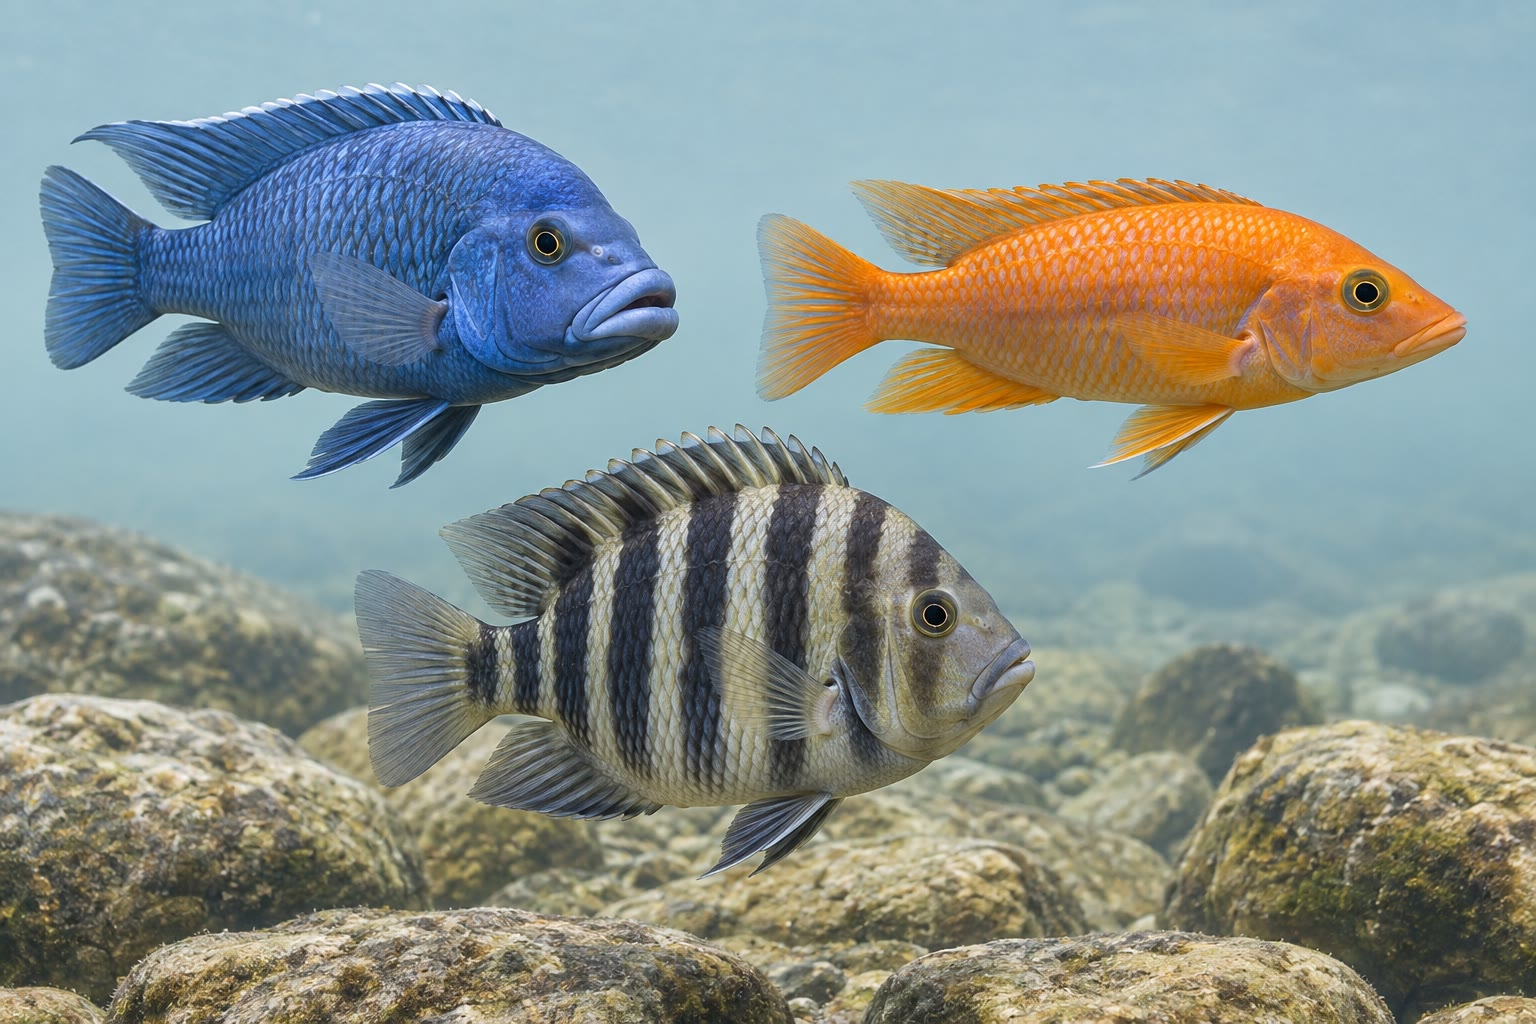
\includegraphics[width=0.44\linewidth]{images/book4/ai/b4-23-cichlids.jpg}

{\small Dua radiasi. Kiri: burung pipit Darwin sebagaimana digambar
Gould pada tahun 1845, satu penjajah menjadi banyak, yang dibedakan
paruhnya. Kanan: ikan siklid sebuah danau Afrika, ratusan spesies dari
beberapa pendiri, yang masing-masing memiliki mulut dan menunya sendiri.}
\end{omfigure}

\section{Makroevolusi: pandangan panjangnya}

\begin{proposition}[Tempo dan modus]\label{prop:b2:speciation:tempo}
\index{kesetimbangan tersela}\index{gradualisme}\index{kepunahan massal}
Sepanjang beberapa lusin generasi ngengatnya berubah warna dan burung
pipitnya berubah paruh; sepanjang jutaan tahun catatan fosilnya
memperlihatkan garis keturunan yang nyaris tidak berubah selama
bentangan yang panjang lalu, dalam sekejap geologis beberapa ribu
tahun, digantikan sebuah keturunan yang khas --- yaitu
\emph{\omterm{prop:b2:speciation:tempo}{kesetimbangan tersela}}, yang merupakan rupa \omterm{prop:b2:speciation:modes}{spesiasi alopatrik} di
dalam populasi tepi yang kecil yang disusul penyebarannya ketika
dicontoh tiap seratus ribu tahun; dan catatannya memperlihatkan garis
keturunan lainnya, kuda di antaranya, yang berubah secara bertahap
sepanjang berlusin-lusin spesies. Di atas spesiesnya, catatannya adalah
catatan pergantian: kebanyakan spesies bertahan satu sampai sepuluh
juta tahun, laju \emph{kepunahan latarnya} adalah kira-kira satu
spesies dari sejuta tiap tahun, dan lima kali --- pada akhir zaman
Ordovisium, Devon, Perm (ketika sembilan persepuluh spesies laut
lenyap), Trias, dan Kapur --- sebuah \emph{\omterm{prop:b2:speciation:tempo}{kepunahan massal}}
menyingkirkan sebagian besar yang hidup dalam beberapa ratus ribu tahun
lalu menyetel ulang permainannya, dengan yang bertahan hidup
berradiasi ke dalam relung yang telah dikosongkan: mamalia ke dalam
dunia dinosaurus setelah asteroid 66 juta tahun yang lalu. Makroevolusi
adalah pola yang telah digambar mikroevolusi pada bab ini dan bab
sebelumnya, yang dijalankan selama waktu yang sangat panjang dan
diselingi bencana.
\end{proposition}

\begin{example}[Perbandingan laju]\label{ex:b2:speciation:rates}
Seleksi pada burung pipitnya mengubah kedalaman paruh sebesar
\qty{4}{\%} dalam satu generasi; seluruh radiasi Galapagosnya, empat
belas spesies dari satu pendiri, memerlukan dua juta tahun; selisih
ukuran tubuh antara seekor mencit dan seekor gajah, yaitu sekitar
$10^{5}$, dapat dihasilkan seleksi sekuat seleksi burung pipitnya dalam
beberapa ratus generasi --- dan catatannya memperlihatkan bahwa ia
memerlukan empat puluh juta tahun. Paradoksnya terselesaikan dengan
memperhatikan bahwa seleksi jarang mendorong ke arah yang sama untuk
waktu yang lama: ia berbalik bersama cuacanya, sebagaimana yang terjadi
di Daphne Major pada tahun setelah kekeringannya, dan \omterm{prop:b2:population-genetics:kinds}{seleksi pemantap}
menahan sebagian besar garis keturunan tetap di tempatnya. Perubahan
yang berkelanjutan itu jarang, dan itulah sebabnya spesiasi, yang
memerlukannya, berjalan lambat --- dan sebabnya, ketika dunianya
berubah cepat, sebagaimana pada \cref{ch:b2:global-change}, garis
keturunan yang tidak dapat mengikutinya hilang.
\end{example}

\section{Latihan}

\begin{exercise}[$\star$]\label{exo:b2:speciation:1}
Nyatakan \omterm{def:b2:speciation:species}{konsep spesies biologis} dan berikan tiga kasus yang padanya ia
tidak dapat diterapkan, beserta konsep yang dipakai sebagai gantinya.
\end{exercise}

\begin{exercise}[$\star$]\label{exo:b2:speciation:2}
Golongkanlah sebagai prazigotik atau pascazigotik: dua ekor katak yang
berbiak pada bulan yang berbeda; seekor bagal; sperma bulu babi yang
tidak dapat mengikat telur spesies lain; tumbuhan hibrida yang gagah
tetapi \omterm{def:b2:angiosperm-reproduction:seed}{bijinya} tidak berkecambah; dua ekor jangkrik yang nyanyiannya
berbeda.
\end{exercise}

\begin{exercise}[$\star$]\label{exo:b2:speciation:3}
Definisikan \omterm{prop:b2:speciation:modes}{spesiasi alopatrik}, peripatrik, simpatrik, dan parapatrik,
beserta sebuah contoh masing-masingnya.
\end{exercise}

\begin{exercise}[$\star$]\label{exo:b2:speciation:4}
Nyatakan keempat hasil \omterm{thm:b2:speciation:lv}{persaingan Lotka--Volterra} dan syarat \omterm{thm:b2:speciation:lv}{hidup
berdampingan} yang mantap dengan kata-kata.
\end{exercise}

\begin{exercise}[$\star\star$]\label{exo:b2:speciation:5}
Dengan $K_1 = 1000$, $K_2 = 800$, $\alpha = 0.5$, $\beta = 0.6$,
hitunglah kerapatan kesetimbangannya lalu periksalah bahwa tiap
spesiesnya dapat menyerbu daya dukung spesies lainnya.
\end{exercise}

\begin{exercise}[$\star\star$]\label{exo:b2:speciation:6}
Dengan $K_1 = 1000$, $K_2 = 800$, $\alpha = 1.5$, $\beta = 0.3$,
spesies mana yang menang, dan mengapa? Bagaimana jika $\alpha = 1.5$ dan $\beta = 1.5$?
\end{exercise}

\begin{exercise}[$\star\star$]\label{exo:b2:speciation:7}
Sebuah tetraploid muncul di dalam sebuah populasi \omterm{def:b2:meiosis-heredity:meiosis}{diploid}. Berikan
jumlah kromosom gametnya, jumlah kromosom sebuah persilangan dengan
\omterm{def:b2:meiosis-heredity:meiosis}{diploidnya}, dan jumlah kromosom gamet hibrida itu, lalu jelaskan
mengapa tetraploidnya terisolasi seketika. Mengapa ia meskipun demikian
biasanya gagal bertahan?
\end{exercise}

\begin{exercise}[$\star\star$]\label{exo:b2:speciation:8}
Dua populasi masing-masing telah memancangkan 10 penggantian sejak
keduanya berpisah, dan tiap pasang \omterm{def:b2:meiosis-heredity:vocabulary}{alel} baru dari kedua sisinya tidak
sesuai dengan peluang $0.01$. Hitunglah jumlah ketaksesuaian harapan
sekarang, dan setelah 30 penggantian masing-masing. Apa yang diramalkan
hal ini bagi hubungan antara pengisolasiannya dan waktunya?
\end{exercise}

\begin{exercise}[$\star\star$]\label{exo:b2:speciation:9}
Hitunglah lebar sebuah \omterm{prop:b2:speciation:reinforcement}{zona hibrida} bagi pemencaran $\sigma =
\qty{2}{km}$ tiap generasi dan kerugian hibrida $s = 0.05$, lalu bagi
$\sigma = \qty{0.3}{km}$ dan $s = 0.4$. Zona mana yang lebih mungkin
berakhir pada penguatan, dan mengapa?
\end{exercise}

\begin{exercise}[$\star\star\star$]\label{exo:b2:speciation:10}
Dua spesies burung pipit bersaing memperebutkan \omterm{def:b2:angiosperm-reproduction:seed}{biji} dengan
$\alpha = \beta = 0.9$ dan $K_1 = K_2 = 500$. Apakah keduanya \omterm{thm:b2:speciation:lv}{hidup berdampingan}?
\omterm{prop:b2:speciation:displacement}{Pergeseran sifat} memperkecil $\alpha$ dan $\beta$ menjadi $0.4$: hitung
ulang kesetimbangannya. Jelaskan dalam istilah isoklinnya apa yang
dikerjakan pergeserannya.
\end{exercise}

\begin{exercise}[$\star\star\star$]\label{exo:b2:speciation:11}
Keluarga Grant menemukan bahwa setelah kekeringan tahun 2004 kedalaman
paruh rerata burung pipit tanah sedangnya turun sebesar \qty{0.7}{mm}
dengan $h^{2} = 0.7$, dengan yang bertahan hidup berparuh \qty{1}{mm}
lebih kecil daripada populasinya. Periksalah tanggapannya dengan
\omterm{thm:b2:population-genetics:heritability}{persamaan pemulia}, lalu jelaskan mengapa kehadiran burung pipit tanah
besarnya, dan bukan kekeringannya saja, yang menyebabkan arah
perubahannya.
\end{exercise}

\begin{exercise}[$\star\star\star$]\label{exo:b2:speciation:12}
``Spesies dibuat secara kebetulan dan dijaga oleh seleksi.'' Bahaslah,
dengan model dua lokusnya, penguatannya, dan peran geografinya.
\end{exercise}

\section{Soal: Dua Burung Pipit di Sebuah Pulau}

\begin{problem}[{Soal akhir pekan --- seekor burung pipit penduduk
berjumpa dengan seekor penyerbu: persaingannya dianalisis pada bidang
fasenya, pergeseran paruh penduduknya diramalkan dari persamaan
pemulia, dan pengisolasian di antara keduanya diukur terhadap sebuah
zona hibrida, berakhir pada kerapatan kesetimbangannya, pergeseran
paruhnya, dan lebar klinanya}]
\label{pb:b2:speciation:1}
Spesies penduduk 1: $K_1 = 1200$, $r_1 = 0.5$ tiap tahun; spesies
penyerbu 2: $K_2 = 400$. Sebelum pergeserannya $\alpha = 0.9$, $\beta =
0.3$; sebuah kekeringan menyetengahkan kedua daya dukungnya selama satu
tahun. Kedalaman paruh spesies 1: rerata \qty{9.5}{mm}, simpangan baku
\qty{0.8}{mm}, $h^{2} = 0.7$. Parameter \omterm{prop:b2:speciation:reinforcement}{zona hibridanya}: $\sigma =
\qty{0.5}{km}$, $s = 0.2$.

\medskip
\noindent\textbf{Bagian I --- Penyerbuannya.}
\begin{enumerate}
  \item Tulislah kedua isoklinnya dan potongannya.
  \item Dapatkah spesies 2 menyerbu spesies 1 pada $K_1$? Dapatkah
        spesies 1 menyerbu spesies 2 pada $K_2$? Simpulkan hasilnya.
  \item Hitunglah kerapatan kesetimbangannya.
  \item Hitunglah $\mathrm{d}N_1/\mathrm{d}t$ pada saat spesies 2 tiba
        dengan $N_2 = 20$ dan $N_1 = 1200$. Apa arti tandanya?
  \item Selama kekeringannya kedua $K$-nya disetengahkan. Hitung ulang
        kesetimbangannya lalu katakan apa yang terjadi pada jumlah tiap
        spesiesnya.
  \item Mengapa efek penyerbunya terhadap penduduknya ($\alpha = 0.9$)
        lebih besar daripada efek penduduknya terhadap penyerbunya
        ($\beta = 0.3$)?
\end{enumerate}

\medskip
\noindent\textbf{Bagian II --- Pergeserannya.}
Pada kekeringannya individu penduduk yang berparuh terbesar paling
bersaing dengan penyerbunya lalu mati: yang bertahan hidup memiliki
paruh rerata \qty{9.0}{mm}.
\begin{enumerate}[resume]
  \item Hitunglah diferensial seleksinya dan tanggapannya.
  \item Berikan paruh rerata generasi berikutnya.
  \item Setelah pergeserannya, $\alpha$ turun menjadi $0.5$. Hitung
        ulang kesetimbangannya (dengan $K$ yang asli).
  \item Jelaskan apa yang dikerjakan pergeserannya terhadap isoklin
        spesies 1.
  \item Jika seleksi sekuat ini bekerja tiap tahun, berapa tahun yang
        diperlukan untuk menggeser paruhnya sebesar \qty{2}{mm}?
        Mengapa hal itu tidak terjadi?
  \item Bandingkan dengan umur radiasinya yang dua juta tahun lalu
        berilah ulasan.
\end{enumerate}

\medskip
\noindent\textbf{Bagian III --- Pengisolasiannya.}
Kedua spesiesnya dapat berhibrida; hibridanya memiliki paruh menengah
dan \omterm{def:b2:population-genetics:fitness}{kebugaran} $1 - s$.
\begin{enumerate}[resume]
  \item Sebutkan penghalang prazigotik yang menjaga hibridisasinya
        tetap jarang pada burung pipit Darwin, dan satu ongkos
        pascazigotik hibridanya.
  \item Hitunglah lebar sebuah \omterm{prop:b2:speciation:reinforcement}{zona hibrida} di antara keduanya bagi $\sigma
        = \qty{0.5}{km}$, $s = 0.2$.
  \item Pulaunya \qty{1}{km} melintang. Apa yang disiratkan hal itu?
  \item Jelaskan bagaimana penguatannya akan berlangsung, dan sifat apa
        yang akan ia kenai.
  \item Dua populasi penduduknya di pulau yang berbeda masing-masing
        telah memancangkan 15 penggantian sejak keduanya berpisah;
        pasangannya tidak sesuai dengan peluang $0.005$. Hitunglah
        ketaksesuaian harapannya lalu katakan apakah keduanya spesies.
  \item Akankah \omterm{def:b2:speciation:species}{konsep spesies biologis}, konsep morfologis, dan konsep
        filogenetik sepakat tentang kedua populasi pulaunya? Jelaskan.
\end{enumerate}

\medskip
\noindent\textbf{Bagian IV --- Pandangan panjangnya.}
\begin{enumerate}[resume]
  \item Jika sebuah spesies bertahan secara rerata 5 juta tahun,
        berapakah laju kepunahan latarnya tiap spesies tiap tahun? Bagi
        sebuah biota berisi 10 juta spesies, berapa kepunahan tiap
        tahun?
  \item Laju kepunahan sekarang ditaksir 100 sampai 1000 kali laju
        latarnya. Berapa spesies tiap tahun itu?
  \item Sebuah \omterm{prop:b2:speciation:tempo}{kepunahan massal} menyingkirkan \qty{75}{\%} spesies
        dalam \num{100000} tahun. Bandingkan lajunya dengan laju
        sekarang.
  \item Jelaskan dalam satu kalimat mengapa yang bertahan hidup dari
        sebuah \omterm{prop:b2:speciation:tempo}{kepunahan massal} berradiasi.
  \item Sebuah garis keturunan di dalam catatannya sedikit berubah
        selama 3 juta tahun, lalu digantikan dalam \num{20000} tahun
        oleh sebuah keturunan yang khas. Sebutkan polanya dan berikan
        modus spesiasi yang menghasilkannya.
  \item Dengan memakai \qty{4}{\%} tiap generasi burung pipitnya,
        berapa generasi seleksi yang berkelanjutan yang akan
        melipatduakan kedalaman paruhnya? Mengapa catatan fosilnya
        memperlihatkan perubahan semacam itu memerlukan jutaan tahun?
  \item Nyatakan hasilnya: hasil dan kesetimbangan persaingannya
        sebelum dan sesudah pergeserannya, pergeseran paruhnya dalam
        satu generasi, dan lebar \omterm{prop:b2:speciation:reinforcement}{zona hibridanya}.
\end{enumerate}
\end{problem}
